\chapter{The Living Soil}\label{ch:b2:living-soil}

Charles Darwin's last book, published the year before he died, was
about earthworms. He had put a chalk marker on a field near his
house in 1842 and dug it up in 1871: it lay eighteen centimetres
down, buried by the castings the worms had brought to the surface
at a rate he measured, weighed, and multiplied --- ten tonnes of
\omterm{def:b2:living-soil:soil}{soil} per acre per year passing through their bodies, so that
``the whole of the superficial mould over any such expanse has
passed, and will again pass, every few years through the bodies of
worms.'' The \omterm{def:b2:living-soil:soil}{soil}, in other words, is not a substrate on which
living things stand but a thing living things make. This chapter
is about that making: how rock becomes \omterm{def:b2:living-soil:soil}{soil} and how slowly, who
lives in it and in what numbers, how dead matter is taken apart and
what is left, how the roots of plants bargain with fungi and
bacteria for what they cannot get alone, and how fast a \omterm{def:b2:living-soil:soil}{soil} that
took ten thousand years to build can be lost.

\section{What soil is}

\begin{definition}[Soil and its horizons]\label{def:b2:living-soil:soil}
\index{soil}\index{soil horizon}\index{humus}\index{weathering}\index{pedogenesis}
\emph{Soil} is the layer of weathered mineral matter, organic
matter, water, air and organisms that covers land and supports
plants: about half its volume is pores, filled with water or air
in changing proportion, and the solid half is mineral grains ---
sand (\qtyrange{0.05}{2}{mm}), silt (\qtyrange{2}{50}{\micro m}) and
clay (under \qty{2}{\micro m}), whose proportions give the
\emph{texture} --- with a few per cent of organic matter that
governs most of its properties. A soil profile shows
\emph{horizons}: the \emph{O} horizon of litter and partly decayed
organic matter at the surface; the dark \emph{A} horizon of mineral
soil mixed with \emph{humus}, the stable, dark, colloidal residue
of decomposition; the \emph{B} horizon below, into which clay,
iron and dissolved matter are washed and where they accumulate;
the \emph{C} horizon of weathered parent rock; and the bedrock. A
soil is made (\emph{pedogenesis}) by five factors --- parent
material, climate, organisms, topography and time --- and it is
made slowly: weathering produces of the order of \qty{0.1}{mm} of
soil a year, so a metre of soil is ten thousand years of work.
\end{definition}

\begin{omfigure}
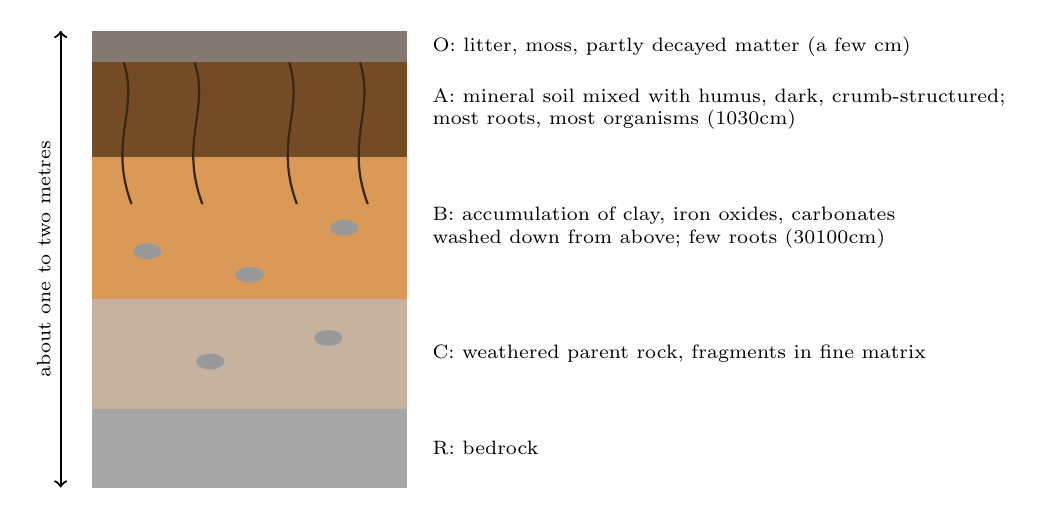
\begin{tikzpicture}[every node/.style={font=\scriptsize}]
  \fill[brown!25!black!60] (0,5.4) rectangle (4,5.8); \node[right] at (4.2,5.6) {O: litter, moss, partly decayed matter (a few cm)};
  \fill[brown!60!black] (0,4.2) rectangle (4,5.4); \node[right, align=left] at (4.2,4.8) {A: mineral soil mixed with humus, dark, crumb-structured;\\ most roots, most organisms (\qtyrange{10}{30}{cm})};
  \fill[brown!70!orange!80] (0,2.4) rectangle (4,4.2); \node[right, align=left] at (4.2,3.3) {B: accumulation of clay, iron oxides, carbonates\\ washed down from above; few roots (\qtyrange{30}{100}{cm})};
  \fill[gray!50!brown!60] (0,1.0) rectangle (4,2.4); \node[right, align=left] at (4.2,1.7) {C: weathered parent rock, fragments in fine matrix};
  \fill[gray!70] (0,0) rectangle (4,1.0); \node[right] at (4.2,0.5) {R: bedrock};
  \foreach \x in {0.4,1.3,2.5,3.4} \draw[brown!30!black, thick] (\x,5.4) .. controls (\x+0.2,4.8) and (\x-0.2,4.4) .. (\x+0.1,3.6);
  \foreach \x/\y in {0.7/3.0, 2.0/2.7, 3.2/3.3, 1.5/1.6, 3.0/1.9} \fill[gray!80] (\x,\y) ellipse (0.18 and 0.1);
  \draw[<->, thick] (-0.4,5.8) -- (-0.4,0) node[midway, left, rotate=90, anchor=south] {about one to two metres};
\end{tikzpicture}

{\small A \omterm{def:b2:living-soil:soil}{soil} profile. Organic matter enters at the top and is
consumed as it descends; mineral matter is released at the bottom
and moved upward by roots and animals; dissolved matter travels
down with the water and is caught in the B horizon.}
\end{omfigure}

\begin{proposition}[Why clay and humus matter]\label{prop:b2:living-soil:cec}
\index{cation exchange capacity}\index{clay}\index{soil structure}\index{field capacity}
Clay particles and \omterm{def:b2:living-soil:soil}{humus} carry negative charges on their surfaces
and hold, by electrostatic attraction, a reserve of exchangeable
cations --- $\mathrm{Ca^{2+}}$, $\mathrm{Mg^{2+}}$, $\mathrm{K^{+}}$, $\mathrm{NH_4^{+}}$ --- that
plant roots draw on by exchanging $\mathrm{H^{+}}$ for them. This
\emph{\omterm{prop:b2:living-soil:cec}{cation exchange capacity}} is the \omterm{def:b2:living-soil:soil}{soil}'s nutrient bank; a sand
has almost none (a few centimoles of charge per kilogram), a clay
loam rich in \omterm{def:b2:living-soil:soil}{humus} fifty times more, and the fertility of the two
differs accordingly. The same surfaces hold water: a sandy \omterm{def:b2:living-soil:soil}{soil}
drains within a day to a \emph{\omterm{prop:b2:living-soil:cec}{field capacity}} of a tenth of its
volume, a loam holds a third, and the difference is what a crop
has between rains. And \omterm{def:b2:living-soil:soil}{humus}, together with fungal hyphae, root
exudates and the mucus of worms, glues mineral grains into
\emph{aggregates}, the crumb structure whose pores let air, water
and roots pass --- the property that distinguishes a \omterm{def:b2:living-soil:soil}{soil} from a
sediment and that is destroyed first by ploughing and compaction.
\end{proposition}

\section{Who lives there}

\begin{proposition}[The soil community]\label{prop:b2:living-soil:community}
\index{soil food web}\index{detritivore}\index{earthworm}\index{soil biomass}
A gram of fertile topsoil holds about $10^{9}$ bacterial cells of
some ten thousand species, a hundred metres of fungal hyphae, $10^{4}$
\omterm{def:b2:unicellular-diversity:protist}{protists}, a few dozen nematodes and a handful of mites and
springtails; a square metre holds a few hundred earthworms and,
below the visible animals, a living mass of several tonnes per
hectare --- comparable to the cattle the same hectare could carry.
The community is a \emph{detrital food web}: bacteria and fungi
(the \emph{decomposers}) eat dead matter and are eaten by \omterm{def:b2:unicellular-diversity:protist}{protists}
and nematodes (the microbial grazers), which are eaten by mites and
predatory nematodes, which feed centipedes and beetles; the
\emph{detritivores} --- earthworms, millipedes, woodlice, termites,
springtails --- eat the litter itself with the microbes on it,
fragmenting it a thousandfold and multiplying the surface the
microbes attack. The grazers matter beyond their numbers: by eating
bacteria they release the nitrogen locked in bacterial cells as
ammonium, and a \omterm{def:b2:living-soil:soil}{soil} with \omterm{def:b2:unicellular-diversity:protist}{protists} and nematodes mineralises
nitrogen faster than one with bacteria alone. Earthworms are the
\emph{ecosystem engineers}: their burrows are the \omterm{def:b2:living-soil:soil}{soil}'s
macropores, their casts are the richest aggregates, and a
grassland's worms move a few tonnes of \omterm{def:b2:living-soil:soil}{soil} per hectare through
their guts each year, as Darwin measured.
\end{proposition}

\begin{omfigure}
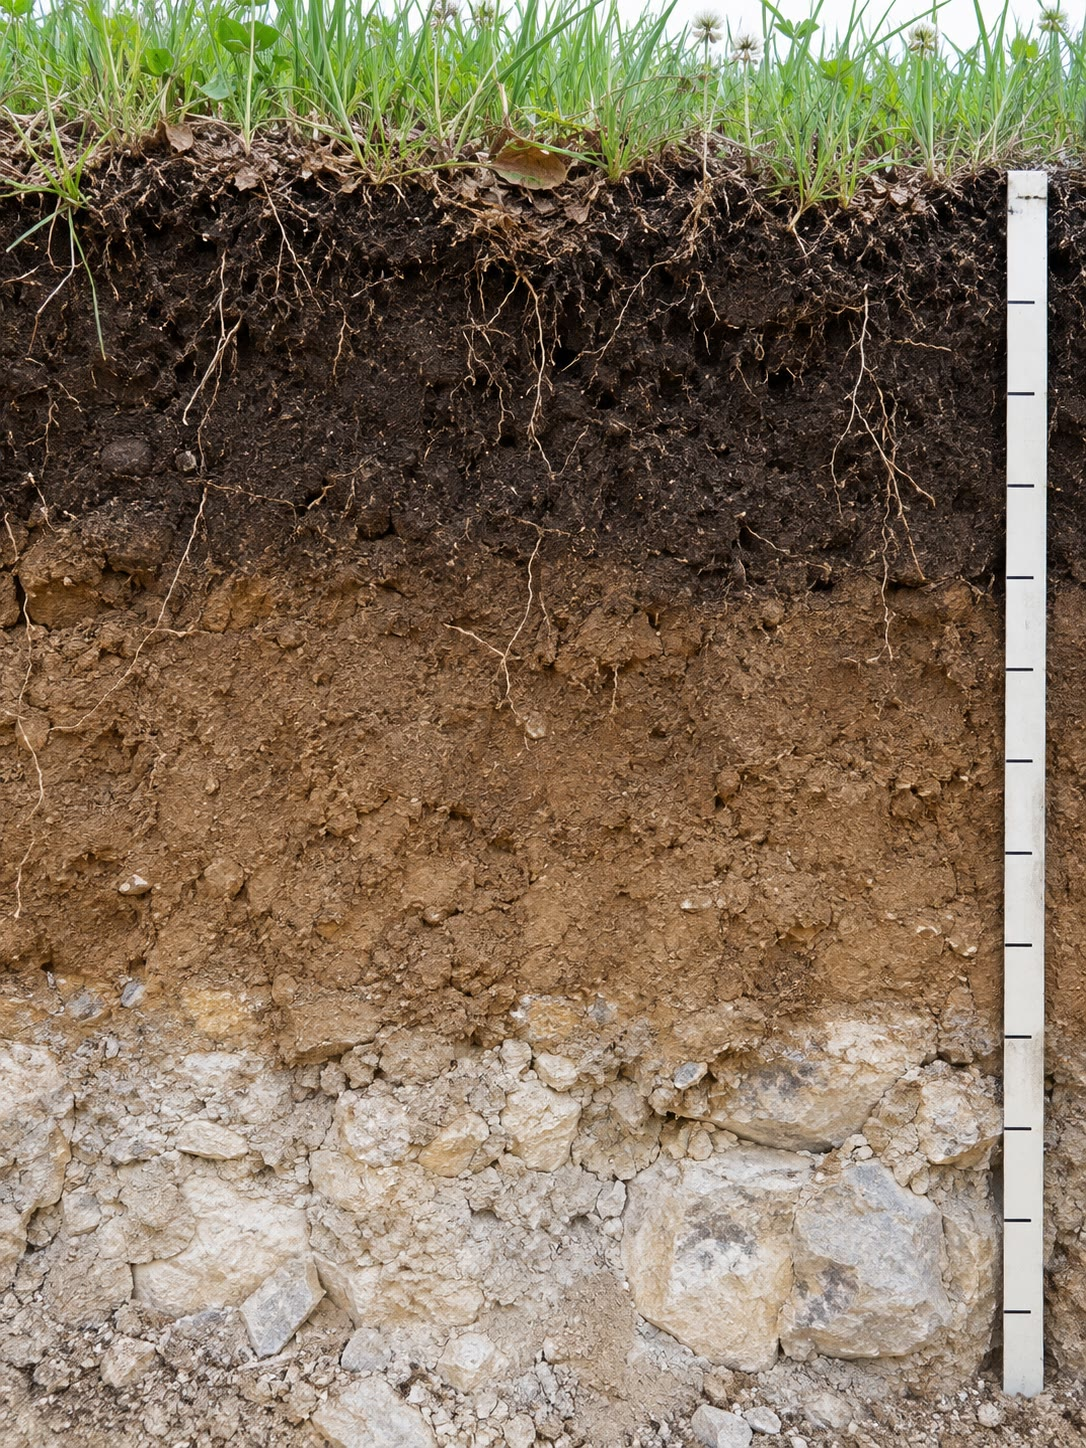
\includegraphics[width=0.21\linewidth]{images/book4/ai/b4-26-soil-profile.jpg}\hspace{0.025\linewidth}
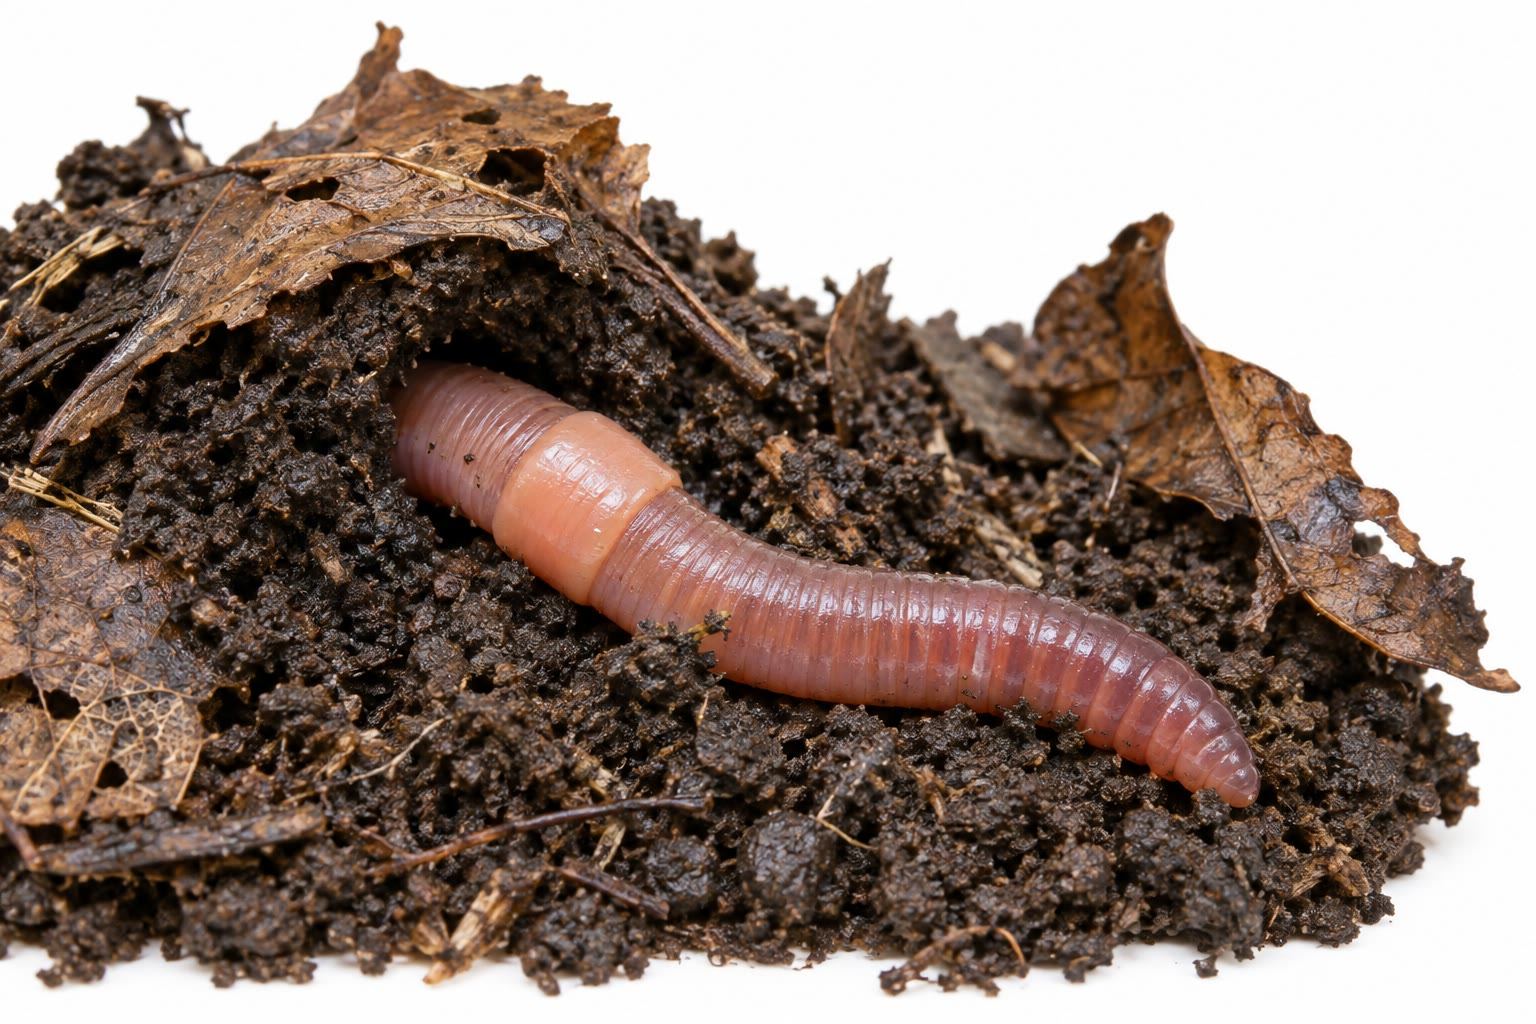
\includegraphics[width=0.42\linewidth]{images/book4/ai/b4-26-earthworm.jpg}\hspace{0.025\linewidth}
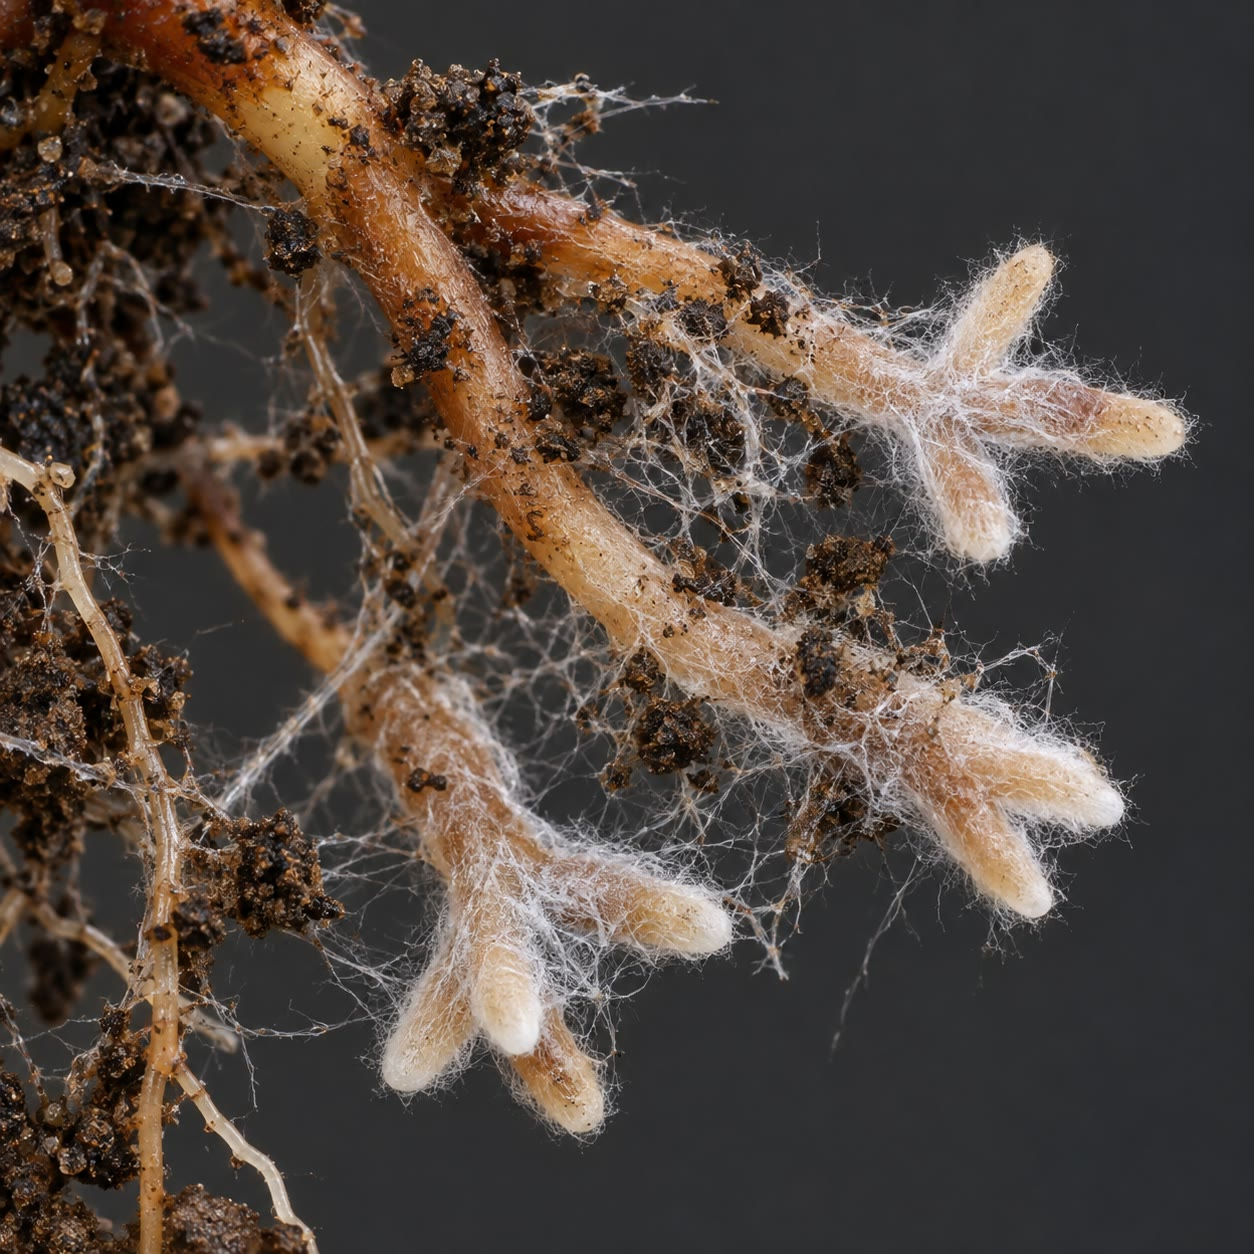
\includegraphics[width=0.28\linewidth]{images/book4/ai/b4-26-mycorrhiza.jpg}

{\small The \omterm{def:b2:living-soil:soil}{soil} and two of its makers. Left: a profile in a cut
bank, dark topsoil grading down to pale weathered rock. Middle: an
earthworm in its burrow. Right: a root with its ectomycorrhizal
sheath and the hyphae that extend it into the \omterm{def:b2:living-soil:soil}{soil}.}
\end{omfigure}

\section{Decomposition}

\begin{theorem}[Litter decay and the carbon-to-nitrogen ratio]\label{thm:b2:living-soil:decay}
\index{decomposition}\index{litter decay}\index{C:N ratio}\index{mineralisation}\index{immobilisation}
Litter decomposes at a rate proportional to what remains,
$\mathrm{d}L/\mathrm{d}t = -kL$, so $L = L_0 e^{-kt}$ with a
\emph{decay constant} $k$ of about 1 per year for grass and
deciduous leaves in a temperate forest, $0.3$ for conifer needles,
several per year in the wet tropics and $0.05$ in the tundra;
a steady input $I$ per year builds a litter layer of $I/k$. Decay
is controlled by temperature, moisture, and the litter's
\emph{quality}: nitrogen content, lignin content, and the ratio of
carbon to nitrogen. Microbes have $\mathrm{C:N} \approx 8$ and
retain about \qty{40}{\%} of the carbon they eat, so they need one
nitrogen for every $8/0.4 = 20$ carbons of food: litter with $\mathrm{C:N}$
below about 25 releases ammonium as it decays
(\emph{mineralisation}), while litter above it --- straw at 80,
\omterm{def:b2:plant-meristems:wood}{wood} at 400 --- makes the microbes take up nitrogen from the \omterm{def:b2:living-soil:soil}{soil}
(\emph{immobilisation}), starving the plants until the carbon has
been respired away and the ratio has fallen. That is why fresh
straw ploughed in depresses a crop, why legume residue feeds it,
and why a compost heap needs both.
\end{theorem}
\begin{proof}
For the ratio: microbes eating litter with $c$ carbons per
nitrogen assimilate $0.4c$ carbons and, to build biomass at
$\mathrm{C:N} = 8$, need $0.4c/8 = c/20$ nitrogens; the litter
supplies 1. If $c < 20$ there is nitrogen to spare, released as
ammonium; if $c > 20$ there is a deficit taken from the \omterm{def:b2:living-soil:soil}{soil}. The
threshold 25 in practice reflects a retention efficiency somewhat
below 0.4. For the litter layer: $\mathrm{d}L/\mathrm{d}t = I - kL$
has \omterm{def:b2:biogeochemical-cycles:reservoir}{steady state} $I/k$, approached with time constant $1/k$; the
\omterm{def:b2:biogeochemical-cycles:reservoir}{residence time} of litter is $1/k$, one year in a beech wood and
twenty in the tundra.
\end{proof}
\begin{proof}[Evidence]
Litter-bag experiments --- known masses of leaves in mesh bags,
buried and weighed at intervals --- gave the exponential law and
its constants across every biome (Olson, 1963), and showed with
different mesh sizes that excluding the \omterm{def:b2:living-soil:soil}{soil} animals halves the
rate: the microbes do the chemistry but the animals set the pace.
Across a continent, the same leaf decays in a year in Georgia and
in eight in Alaska, in proportion to actual evapotranspiration,
the product of warmth and water.
\end{proof}

\begin{omfigure}
\begin{tikzpicture}
\begin{axis}[
  width=0.72\linewidth, height=5.6cm,
  axis x line=bottom, axis y line=left,
  xmin=0, xmax=6, ymin=0, ymax=105,
  xlabel={years}, ylabel={litter mass remaining (\%)},
  xlabel style={font=\small, at={(axis description cs:0.5,-0.13)}, anchor=north},
  ylabel style={font=\small},
  tick label style={font=\small},
  legend style={font=\scriptsize, at={(0.5,-0.3)}, anchor=north, draw=none, legend columns=2},
  clip=false,
]
\addplot[very thick, omDef, domain=0:6, samples=60] {100*exp(-2*x)};
\addlegendentry{tropical forest leaf, $k = 2$}
\addplot[very thick, omThm, domain=0:6, samples=60] {100*exp(-1*x)};
\addlegendentry{beech leaf, $k = 1$}
\addplot[very thick, omProp, domain=0:6, samples=60] {100*exp(-0.3*x)};
\addlegendentry{spruce needle, $k = 0.3$}
\addplot[very thick, gray, domain=0:6, samples=60] {100*exp(-0.05*x)};
\addlegendentry{tundra moss, $k = 0.05$}
\end{axis}
\end{tikzpicture}

{\small Exponential decay of litter. Half of a beech leaf is gone
in eight months; half of a tundra \omterm{def:b2:plant-life-cycles:moss}{moss} in fourteen years; the
residue that neither microbe nor animal can finish becomes \omterm{def:b2:living-soil:soil}{humus}.}
\end{omfigure}

\begin{proposition}[Humus and the soil carbon pool]\label{prop:b2:living-soil:humus}
\index{humus}\index{soil organic carbon}\index{soil respiration}
A few per cent of the litter's carbon escapes complete oxidation
and becomes \emph{\omterm{def:b2:living-soil:soil}{humus}}: a dark, amorphous mixture of microbial
residues, altered lignin and plant compounds, bound to clay and
iron and locked in aggregates, that decays with \omterm{def:b2:biogeochemical-cycles:reservoir}{residence times} of
decades to millennia. \omterm{def:b2:living-soil:soil}{Humus} is where the \omterm{def:b2:living-soil:soil}{soil}'s fertility lives
--- most of its nitrogen and cation exchange, half its water-holding
--- and it is the largest pool of organic carbon on land,
\qty{1700}{GtC} in the top metre, twice the atmosphere's. Its
balance is input minus decay, $\mathrm{d}H/\mathrm{d}t = I_h - k_hH$:
with $k_h \approx 0.02$ per year a \omterm{def:b2:living-soil:soil}{soil} holds fifty years' input,
and any change --- ploughing, which breaks the aggregates and
aerates the \omterm{def:b2:living-soil:soil}{humus}; drainage of a peat, which admits oxygen;
warming, which raises $k_h$ --- shows up as a loss that continues
for decades. The world's cultivated \omterm{def:b2:living-soil:soil}{soils} have lost a third to a
half of their \omterm{def:b2:living-soil:soil}{humus} since they were first broken, some
\qty{100}{GtC}, and a warming of \qty{3}{\celsius} would raise the
decay of the rest by a third: \omterm{def:b2:living-soil:soil}{soils} are the largest uncertainty in
the carbon budget of \cref{ch:b2:global-change}.
\end{proposition}

\section{Partnerships below ground}

\begin{proposition}[Mycorrhizae and rhizobia]\label{prop:b2:living-soil:symbiosis}
\index{mycorrhiza}\index{rhizobium}\index{root nodule}\index{nitrogenase}\index{leghaemoglobin}
Nine plant species in ten have their roots colonised by fungi in a
\emph{mycorrhiza}: the plant gives sugar (a tenth to a fifth of its
photosynthate) and the fungus gives phosphate, nitrogen, water and
zinc, which its hyphae, a hundred times thinner than a root and
extending a hundred times its length per unit of carbon, collect
from a \omterm{def:b2:living-soil:soil}{soil} volume the root cannot reach --- phosphate in
particular, which diffuses so slowly through \omterm{def:b2:living-soil:soil}{soil} that a root
exhausts its millimetre of neighbourhood within days.
\emph{Arbuscular} mycorrhizae, the older kind, enter the root cells
and branch into arbuscules where the exchange takes place;
\emph{ectomycorrhizae} of forest trees sheath the root tip and
grow between its cells. Legumes go further: rhizobia, attracted by
the root's flavonoids, enter through a \omterm{prop:b2:plant-meristems:ram}{root hair}, and the root
builds a \emph{nodule} around them in which the bacteria, as
\emph{bacteroids}, fix nitrogen with nitrogenase --- an enzyme so
sensitive to oxygen that the nodule must be kept nearly anoxic by
\emph{leghaemoglobin}, a haemoglobin the plant makes, which gives
the nodule its pink colour and delivers oxygen to the bacteroids
at a concentration too low to poison the enzyme. Each partner
polices the other: a plant cuts off sugar to nodules that fix
nothing, and a fungus that delivers less phosphate receives less
carbon.
\end{proposition}
\begin{proof}[Evidence]
Kiers and colleagues (2011) grew a plant with two fungal partners
on a divided root system and offered phosphate to one side only:
the plant allocated more carbon to the fungus that supplied more
phosphate, and the fungus allocated more phosphate to a root that
gave more carbon --- reciprocal rewards measured with isotopes.
For rhizobia, nodules experimentally denied nitrogen (by
replacing the air with argon and oxygen) received less oxygen and
grew less than nodules on the same plant that could fix: the plant
sanctions cheaters. Nitrogen-15 tracing shows that a clover--grass
sward transfers a third of the clover's fixed nitrogen to the
grass within a season, through the \omterm{def:b2:living-soil:soil}{soil} and through shared fungal
networks.
\end{proof}

\begin{omfigure}
\begin{tikzpicture}[every node/.style={font=\scriptsize}, >=stealth]
  % root cross-section
  \fill[omThm!15] (0,0) circle (1.5); \draw[thick] (0,0) circle (1.5);
  \fill[omThm!30] (0,0) circle (0.5); \draw[thick] (0,0) circle (0.5);
  \node at (0,0) {stele};
  \node at (0,1.05) {cortex};
  % arbuscules in cortex cells
  \foreach \a in {30,150,270} { \draw[omDef, thick] ({1.0*cos(\a)},{1.0*sin(\a)}) -- ++({0.25*cos(\a+60)},{0.25*sin(\a+60)}) -- ++({0.2*cos(\a-40)},{0.2*sin(\a-40)}); \draw[omDef, thick] ({1.0*cos(\a)},{1.0*sin(\a)}) -- ++({0.25*cos(\a-60)},{0.25*sin(\a-60)}); }
  % hyphae out
  \foreach \a in {20,80,150,210,340} { \draw[omDef, thick] ({1.5*cos(\a)},{1.5*sin(\a)}) .. controls ({2.2*cos(\a+10)},{2.2*sin(\a+10)}) .. ({2.7*cos(\a-5)},{2.7*sin(\a-5)}); }
  \draw[omDef, thick] ({1.5*cos(150)},{1.5*sin(150)}) -- ({1.0*cos(150)},{1.0*sin(150)});
  \node[omDef, anchor=west, align=left] at (2.9,1.4) {hyphae: \qty{3}{\micro m} wide,\\ metres per centimetre of root};
  \node[omDef, anchor=west] at (2.9,0.1) {arbuscule inside a cortex cell};
  \draw[omDef] (2.85,0.1) -- (1.2,0.5);
  \node[anchor=north, align=center] at (0,-1.6) {root, \qty{0.3}{mm} across};
  \draw[->, thick, omThm] (-1.2,-2.4) -- (1.2,-2.4) node[right] {sugar to the fungus, \qtyrange{10}{20}{\%} of photosynthate};
  \draw[<-, thick, omDef] (-1.2,-2.9) -- (1.2,-2.9) node[right] {phosphate, ammonium, water, zinc to the plant};
  % nodule
  \begin{scope}[xshift=9.3cm]
    \draw[thick, brown!60!black] (-0.3,2.4) -- (-0.1,-0.6);
    \draw[thick, brown!60!black] (-0.1,0.3) -- (1.6,0.1);
    \fill[pink!60!red!40] (1.5,0.2) circle (0.9); \draw[thick] (1.5,0.2) circle (0.9);
    \fill[pink!80!red!60] (1.5,0.2) circle (0.55);
    \foreach \p in {(1.3,0.3),(1.6,0.0),(1.5,0.45),(1.7,0.3),(1.35,0.05)} \fill[omDef!70!black] \p ellipse (0.08 and 0.05);
    \node[anchor=north, align=center] at (1.5,-0.8) {nodule: bacteroids in plant cells,\\ pink with leghaemoglobin;\\ oxygen held at \qty{10}{nM}, so nitrogenase\\ works and the cells still respire};
    \node[anchor=south, align=center] at (-0.2,2.45) {legume root};
  \end{scope}
\end{tikzpicture}

{\small Two bargains. Left: an arbuscular mycorrhiza, sugar out
and phosphate in through arbuscules inside the cortex cells. Right:
a legume nodule, where the plant's own haemoglobin keeps oxygen
low enough for nitrogenase and high enough for respiration.}
\end{omfigure}

\section{Losing soil}

\begin{proposition}[Erosion, salt and the balance of a soil]\label{prop:b2:living-soil:erosion}
\index{soil erosion}\index{salinisation}\index{desertification}
\omterm{def:b2:living-soil:soil}{Soil} forms at \qtyrange{0.05}{0.5}{mm} a year and, under natural
vegetation, erodes at about the same rate. Bare ploughed land on a
slope loses \qtyrange{1}{10}{mm} a year to water and wind ---
\qtyrange{10}{100}{t/ha} --- ten to a hundred times the rate of
formation: a \omterm{def:b2:living-soil:soil}{soil} built in ten thousand years is removed in a
century, and with it the \omterm{def:b2:living-soil:soil}{humus} and the nutrients of the A horizon,
the only part that matters. Cover crops, terraces, contour ploughing
and no-till farming, which leaves the residue on the surface and the
aggregates intact, bring the loss back near the rate of formation.
Irrigation in dry climates brings the opposite failure: water
evaporates and leaves its salts, a tonne per hectare per year from
water that is only slightly saline, until the osmotic potential of
the \omterm{def:b2:living-soil:soil}{soil} solution (\cref{ch:b2:plant-plasticity}) is lower than the
roots can overcome --- \emph{salinisation}, which retired the
fields of Sumer four thousand years ago and now affects a fifth of
irrigated land. The state of a \omterm{def:b2:living-soil:soil}{soil} is a budget: \omterm{def:b2:living-soil:soil}{humus} in against
\omterm{def:b2:living-soil:soil}{humus} out, formation against erosion, salt in against salt
drained; each has a \omterm{def:b2:biogeochemical-cycles:reservoir}{residence time}, and each, once negative, is
slow to reverse.
\end{proposition}

\section{Exercises}

\begin{exercise}[$\star$]\label{exo:b2:living-soil:1}
Name the horizons of a \omterm{def:b2:living-soil:soil}{soil} profile from the surface down and say
what happens in each.
\end{exercise}

\begin{exercise}[$\star$]\label{exo:b2:living-soil:2}
Explain what \omterm{prop:b2:living-soil:cec}{cation exchange capacity} is, why a sandy \omterm{def:b2:living-soil:soil}{soil} has
little, and what a farmer who limes an acid \omterm{def:b2:living-soil:soil}{soil} is doing to it.
\end{exercise}

\begin{exercise}[$\star$]\label{exo:b2:living-soil:3}
List the main groups of the \omterm{prop:b2:living-soil:community}{soil food web} from decomposers to top
predators, with one organism each, and say what the grazers of
bacteria do for the plants.
\end{exercise}

\begin{exercise}[$\star$]\label{exo:b2:living-soil:4}
Distinguish arbuscular and ectomycorrhizae, and state what each
partner gives and gets.
\end{exercise}

\begin{exercise}[$\star\star$]\label{exo:b2:living-soil:5}
A beech forest drops \qty{4}{t/ha} of leaves a year and its \omterm{thm:b2:living-soil:decay}{litter
decays} with $k = 0.8$ per year. Compute the steady-state litter
mass, the litter's \omterm{def:b2:biogeochemical-cycles:reservoir}{residence time}, and the time for a year's fall
to lose \qty{90}{\%} of its mass.
\end{exercise}

\begin{exercise}[$\star\star$]\label{exo:b2:living-soil:6}
Wheat straw has $\mathrm{C:N} = 80$ and clover residue $15$. For
each, compute the nitrogen the microbes need per \qty{100}{kg} of
carbon consumed (retention 0.4, microbial $\mathrm{C:N} = 8$) and
whether the residue mineralises or immobilises, and how much.
\end{exercise}

\begin{exercise}[$\star\star$]\label{exo:b2:living-soil:7}
A hectare of grassland holds \qty{2}{t} of earthworms that each
process ten times their mass of \omterm{def:b2:living-soil:soil}{soil} a year. Compute the \omterm{def:b2:living-soil:soil}{soil}
passed through worms per year and the time for the top
\qty{20}{cm} (bulk density \qty{1.3}{t/m^3}) to pass through once.
Compare with Darwin's figure.
\end{exercise}

\begin{exercise}[$\star\star$]\label{exo:b2:living-soil:8}
A gram of \omterm{def:b2:living-soil:soil}{soil} holds $10^{9}$ bacteria of mass \qty{e-12}{g} each,
and \qty{100}{m} of hyphae of diameter \qty{4}{\micro m} and density
\qty{1.1}{g/cm^3}. Compute the bacterial and fungal biomass per
gram and per hectare (top \qty{20}{cm}, \qty{1.3}{t/m^3}).
\end{exercise}

\begin{exercise}[$\star\star$]\label{exo:b2:living-soil:9}
\omterm{def:b2:living-soil:soil}{Soil} \omterm{def:b2:living-soil:soil}{humus} decays with $k_h = 0.02$ per year and receives
\qty{1.5}{t/ha} of carbon a year. Compute the steady-state \omterm{def:b2:living-soil:soil}{humus}
carbon. The field is ploughed and $k_h$ doubles: compute the new
\omterm{def:b2:biogeochemical-cycles:reservoir}{steady state}, the carbon lost, and the time to lose half of it.
\end{exercise}

\begin{exercise}[$\star\star\star$]\label{exo:b2:living-soil:10}
Phosphate diffuses through \omterm{def:b2:living-soil:soil}{soil} with $D \approx \qty{e-13}{m^2/s}$.
Compute how far it travels in a growing season of \num{100} days
($x \approx \sqrt{2Dt}$) and compare with the spacing of roots
(\qty{1}{cm}) and of hyphae (\qty{0.1}{mm}). What does this say
about why mycorrhizae matter for phosphorus and less for nitrate
($D \approx \qty{e-10}{m^2/s}$)?
\end{exercise}

\begin{exercise}[$\star\star\star$]\label{exo:b2:living-soil:11}
A slope loses \qty{20}{t/ha} of \omterm{def:b2:living-soil:soil}{soil} a year to erosion while
forming \qty{1}{t/ha}; the A horizon is \qty{25}{cm} thick at
\qty{1.3}{t/m^3} and holds \qty{3}{\%} carbon. Compute the A
horizon's mass, its lifetime at this rate, and the carbon lost per
year. Under no-till the loss falls to \qty{2}{t/ha}: recompute the
lifetime.
\end{exercise}

\begin{exercise}[$\star\star\star$]\label{exo:b2:living-soil:12}
``The \omterm{def:b2:living-soil:soil}{soil} is the slowest organism on the farm.'' Discuss with the
\omterm{def:b2:biogeochemical-cycles:reservoir}{residence times} of litter, \omterm{def:b2:living-soil:soil}{humus}, mineral \omterm{def:b2:living-soil:soil}{soil} and salt, and say
which changes a farmer can see within a career and which not.
\end{exercise}

\section{Problem: A Hectare of Soil}

\begin{problem}[{Weekend problem --- one hectare of arable soil
audited: its living mass counted, its litter and humus followed
through their exponential budgets, the nitrogen released by a
legume residue computed against a crop's need, and the erosion and
carbon accounts of two management regimes compared, ending on the
soil's carbon stock, its lifetime under the plough, and the
nitrogen a legume supplies}]
\label{pb:b2:living-soil:1}
The hectare: A horizon \qty{25}{cm} thick, bulk density
\qty{1.3}{t/m^3}, \qty{2.5}{\%} organic carbon; \omterm{def:b2:living-soil:soil}{humus} decay $k_h =
0.025$ per year under the plough, $0.015$ under no-till; carbon
input to the \omterm{def:b2:living-soil:soil}{humus} \qty{1.2}{t/ha} a year in both. Litter: a
clover cover crop leaves \qty{5}{t/ha} of dry matter at
\qty{45}{\%} carbon and \qty{3}{\%} nitrogen, decaying with $k = 2$
per year. Erosion: \qty{15}{t/ha} a year ploughed, \qty{1.5}{t/ha}
no-till; formation \qty{0.5}{t/ha}.

\medskip
\noindent\textbf{Part I --- The stock.}
\begin{enumerate}
  \item Compute the mass of the A horizon and its organic carbon.
  \item Compute the mass of nitrogen in the \omterm{def:b2:living-soil:soil}{humus} if its
        $\mathrm{C:N}$ is 12.
  \item The \omterm{def:b2:living-soil:soil}{soil} holds $10^{9}$ bacteria per gram at \qty{e-12}{g}
        each and \qty{200}{m} of hyphae per gram at \qty{4}{\micro m}
        diameter, density 1.1. Compute the microbial biomass per
        hectare.
  \item Add \qty{1.5}{t/ha} of earthworms and \qty{0.2}{t/ha} of
        other animals, and give the total living mass per hectare.
        What is it as a fraction of the \omterm{def:b2:living-soil:soil}{humus} carbon?
  \item The microbes turn over their biomass twice a year and
        respire \qty{60}{\%} of what they eat. Estimate the carbon
        they consume per year, and the $\mathrm{CO_2}$ respired.
  \item Compare with the crop's net primary production of about
        \qty{5}{t/ha} of carbon and comment.
\end{enumerate}

\medskip
\noindent\textbf{Part II --- The clover residue.}
\begin{enumerate}[resume]
  \item Compute the carbon and nitrogen in the residue and its
        $\mathrm{C:N}$.
  \item With microbial $\mathrm{C:N} = 8$ and retention $0.4$, does
        the residue mineralise or immobilise nitrogen? Compute the
        net nitrogen released as the whole residue decays.
  \item With $k = 2$, what fraction of the residue has decayed after
        3 months? After a year?
  \item Compute the nitrogen released in the first 3 months.
  \item A wheat crop takes up \qty{150}{kg} of nitrogen per hectare,
        most of it in the two months after sowing. Comment on the
        timing.
  \item The same mass of wheat straw ($\mathrm{C:N} = 80$) is
        ploughed in instead. Compute the nitrogen immobilised and
        say what the farmer must do.
\end{enumerate}

\medskip
\noindent\textbf{Part III --- \omterm{def:b2:living-soil:soil}{Humus}.}
\begin{enumerate}[resume]
  \item Compute the steady-state \omterm{def:b2:living-soil:soil}{humus} carbon under the plough and
        under no-till.
  \item The field, at the ploughed \omterm{def:b2:biogeochemical-cycles:reservoir}{steady state}, is converted to
        no-till. Write $H(t)$ and compute the carbon gained after
        10 and 50 years.
  \item Compute the rate of gain in the first year, in tonnes of
        carbon per hectare, and as tonnes of $\mathrm{CO_2}$.
  \item If the world's \qty{1.5e9}{ha} of cropland did the same,
        what would the first-year sink be, against fossil emissions
        of \qty{10}{GtC}? And in the fiftieth year?
  \item Why is the sink temporary and reversible?
  \item A warming of \qty{3}{\celsius} raises $k_h$ by a third.
        Compute the new no-till \omterm{def:b2:biogeochemical-cycles:reservoir}{steady state} and the carbon lost.
\end{enumerate}

\medskip
\noindent\textbf{Part IV --- Erosion.}
\begin{enumerate}[resume]
  \item Compute the net loss of \omterm{def:b2:living-soil:soil}{soil} per year under each regime.
  \item Compute the lifetime of the A horizon under each.
  \item Compute the carbon and nitrogen carried off per year by
        erosion under the plough.
  \item Compare the erosion carbon loss with the \omterm{def:b2:living-soil:soil}{humus} decay loss at
        \omterm{def:b2:biogeochemical-cycles:reservoir}{steady state} under the plough.
  \item The eroded \omterm{def:b2:living-soil:soil}{soil} is deposited downstream. Is its carbon
        lost to the atmosphere? Discuss.
  \item Give the \omterm{def:b2:biogeochemical-cycles:reservoir}{residence times} of litter, \omterm{def:b2:living-soil:soil}{humus} and mineral \omterm{def:b2:living-soil:soil}{soil}
        on this hectare.
  \item State the result: the A horizon's carbon stock, its
        lifetime under the plough and under no-till, and the
        nitrogen the clover residue supplies.
\end{enumerate}
\end{problem}
